%!TEX root = ./icml2016.tex
\section{Bayesian RESCAL}

For each entity $i$, $e_i \in \mathbb{R}^{D}$ is drawn from multivariate-normal distribution. Let $E$ be a $I \times D$ matrix representation of entities.
\begin{align}
\label{eqn:entity_gen}
e_i \sim {N}(\mathbf{0}, \sigma_e^2{I}_D)
\end{align}
For each relation $k$, we draw matrix $R_k \in \mathbb{R}^{D\times D}$ from zero-mean matrix normal distribution.
\begin{align}
\label{eqn:relation_gen}
R_k \sim \mathcal{N}_{D \times D}(\mathbf{0}, \sigma_r{I}_D, \sigma_r{I}_D) \\
\text{vec}(R_k) = r_k \sim N(\mathbf{0}, \sigma_r^2 I_{D^2})
\end{align}
For each triple $(i,k,j)$, we draw $x_{ikj}$
\begin{align}
\label{eqn:triple_gen}
x_{ikj} |e_i, e_j, R_k &\sim \mathcal{MN}(e_i^{\top} R_k e_j, \sigma_x^2)\\
& = \mathcal{N}(r_k^{\top} e_i \otimes e_j, \sigma_x^2)
\end{align}


%\begin{figure}[t]
%	\centering
%	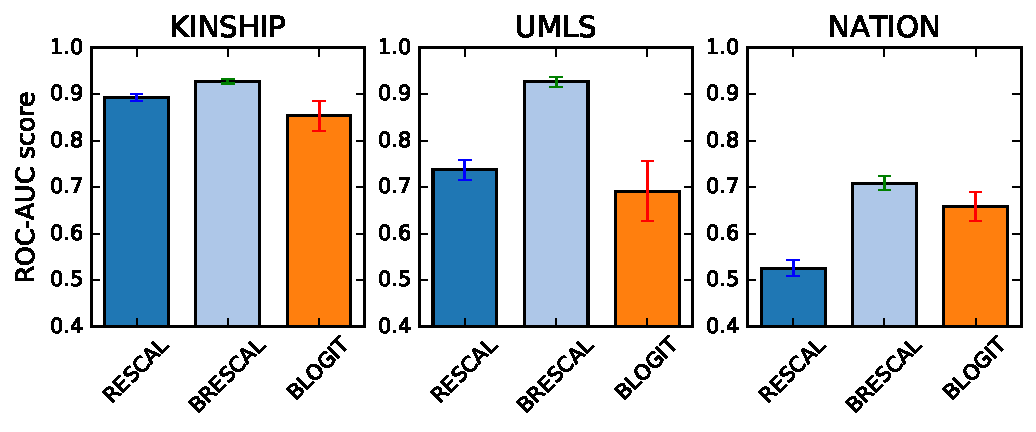
\includegraphics[width=\linewidth]{images/rescal_vs_brescal.pdf}			
%	\caption{\label{fig:r_vs_br} ROC-AUC scores on three different datasets. BRESCAL and BLOGIT represent Bayesian RESCAL and Bayesian RESCAL with logistic regression outputs, respectively. BRESCAL consistently outperforms RESCAL across all datasets.}
%\end{figure}


%For binary valued triples (Logistic regression):
%\begin{align}
%p(x_{ikj}=1) = \sigma(e_i^{\top} R_k e_j, \sigma_x^2)
%\end{align}

